%%%%Use this as a filler to get the template working
%%Introduction
\chapter{Introduction}
The Standard Model (SM) is the culmination of more than a century of work. The first piece added to the puzzle was the electron, discovered in 1891. Since then, 24 other particles have been discovered, with the final piece, the Higgs Boson, being added in 2012. Since it was theorized, the SM has held up to rigorous experimentation and remains an unbeaten theory of fundamental matter and forces. Even though the SM is widely successful, it fails to explain all observed phenomena. Gravity, neutrino masses, dark matter, along with other observations, all lack explanation within the SM. The remaining task is to probe the extremes of the SM to either more precisely measure the parameters or to find its limit.
%Include this is a search for BSM production
\section{The Standard Model}
The Standard Model defines the basic building blocks of matter and force and the interactions between them. Everyday matter is made of protons, neutrons, and electrons. Electrons are a fundamental particle, called a lepton, meaning they are not made of smaller constituents. However, protons and neutrons are not fundamental particles. They are a composite of up and down quarks, two more fundamental particles. The protons are made of two ups and a down and the neutrons are made of two downs and an up. The up and down quarks, along with the electron, are types of fermions. \newline
\indent Fermions are spin-${\frac{1}{2}}$ particles that make up all matter in the SM. The fermions can be broken down into 3 ``generations". Where a generation contains two quarks, one with electric charge ${+\frac{2}{3}}$ and one with electric charge ${-\frac{1}{3}}$, one electrically charged lepton, charge -1, and one electrically neutral lepton. The quarks have an additional color charge, of which there are 3 charges. This is additional quantum number associated with the strong force. In all, this gives 12 fermions. \newline 

\begin{table}[h]
\begin{center}
\footnotesize
\begin{tabular}[h]{|c||c|c|c|c|}
\hline
 & Particle & Spin & Charge & Mass \\
\hline\hline
Quarks &&&&\\
\hline
u type &u& & &${2.4^{+0.6}_{-0.4} MeV}$\\
 &c&${\frac{1}{2}}$&${\frac{2}{3}}$&${1.28\pm{0.03} GeV}$\\
 &t& & &${173.1\pm{0.6} GeV}$\\
\hline
d type & d& & & ${4.7^{+0.5}_{-0.4} MeV}$\\
 & s & ${\frac{1}{2}}$ & ${-\frac{1}{3}}$ & ${96^{+8}_{-4} MeV}$\\
 & b & & & ${4.18^{+0.04}_{-0.03} GeV}$\\
\hline\hline
Leptons &&&&\\
\hline
e family & e & ${\frac{1}{2}}$ & -1 &${0.5109989461\pm{}0.000000003 MeV}$\\
 & ${\nu_{e}}$ & & 0 & ${< 2 eV}$\\
 \hline
${\mu}$ family & ${\mu}$ & ${\frac{1}{2}}$ & -1 &${105.6583745\pm{}0.0000024 MeV}$\\
 & ${\nu_{\mu}}$ & & 0 & ${< 2 eV}$\\
 \hline
${\tau}$ family & ${\tau}$ & ${\frac{1}{2}}$ & -1 &${1776.86\pm{}0.12 GeV}$\\
 & ${\nu_{\tau}}$ & & 0 & ${< 2 eV}$\\
 \hline\hline
 Bosons &&&&\\
 \hline
 Vector & ${\gamma}$ & 1 & 0 & ${< 10^{-18} eV}$\\
 & ${g}$ & 1 & 0 & ${0}$\\
 & ${W}$ & 1 & ${\pm}$ & ${80.385\pm{}0.0015 GeV}$\\
 & ${Z}$ & 1 & 0 & ${91.1876\pm{}0.0021 GeV}$\\
 \hline
 Scalar & H & 0& 0 & ${125.09\pm{}0.21\pm{}0.11 GeV}$\\
 \hline
\end{tabular}
\caption[Particles of the Standard Model]{Particles of the Standard Model ~\cite{PhysRevD.98.030001}}
\label{tab:SM}
\end{center}
\end{table}

\indent Gauge bosons are spin-${1}$ particles responsible for carrying the fundamental forces in the standard model. There are 12 physical gauge bosons. The photon ${\gamma}$ is a massless, charge neutral force carrier for the electromagnetic force. The nuclear forces are carried by 3 massive gauge bosons. A chargeless Z boson and two charged W bosons, ${Charge = \pm 1}$. Together, these four bosons control the electroweak interactions in the standard model. The remaining 8 bosons are the gluons, the force carriers for the strong nuclear interaction. Gluons are massless, electrically neutral particles that have two color charges. There is a gluon for each linearly independent combination of the three color, anti-color, charges, giving the 8 colored gluons. The color singlet state does not exist in SU(3).\newline
\indent The remaining piece of the standard is the Higgs Boson. The Higgs boson is a massive scalar, spin-${0}$, chargeless boson. The Higgs boson is responsible for giving mass to the massive fundamental particles. The full list of SM particles and their properties are in Table ~\ref{tab:SM}\newline
\indent. Along with all of the fundamental particles, there are also anti-particles. Every particle in the SM has a partner of identical mass but opposite charge. These anti-particles, when they interact with their matching particle, annihilate. For example, the anti-particle to the electron is the positron; a particles with electric charge of -1. For the W boson, the positive and negative Ws are particle-antiparticle pairs. Some particles are their own anti particle, known as Majorana particles. For example, the anti-particle of a photon is a photon, the same is true for the Z boson.\newline
\subsection{Interactions}
The SM is governed by three different types of interactions. For leptons, the overarching theory is the electroweak theory. This can be broken down further into the electromagnetic interaction, Quantum Electrodynamics (QED) and the weak interaction. The electromagnetic interaction defines the interaction of electrically charged particles with photons. The fundamental diagram for the electromagnetic interaction is electron-positron annihilation figure ~\ref{Fey:e-p}, where an electron and a positron collide and produce two photons. This can also be reversed, two photons interact and produce an electron-positron pair. The strength of this interaction is the electrical charge e. \newline

\begin{figure}[h]
\begin{center}
\begin{tikzpicture}
\begin{feynman}
\vertex (c) ;
\vertex [below left =of c] (i1){\(e^{-}\)};
\vertex [above left=of c] (i2) {\(e^{+}\)};
\vertex [below right=of c] (f1){\(\gamma\)};
\vertex [above right= of c] (f2){\(\gamma\)};
\diagram* {
(i1) -- [fermion] (c) -- [fermion] (i2) ,
(f1) -- [photon] (c)-- [photon] (f2)
};
\end{feynman}
\end{tikzpicture}
\caption[Electron-Positron Annihilation]{Electron-Positron Annihilation}
\label{Fey:e-p}
\end{center}
\end{figure}

\indent The weak interaction defines the interaction of particles under the weak isospin quantum number. In the SM, every fermion is a mix of a left and a right-handed chirality. Particle with a right-handed chirality have a weak isospin T = 0. These particles exist as singlets and do not interact with the weak force. Left-handed particles have a weak isospin T =  ${\frac{1}{2}}$. These particles live as doublets as illustrated in table ~\ref{tab:chiral}. For these particles, the third component of the weak isospin T\textsubscript{3}, ${+\frac{1}{2}}$ for up-type quarks and charged leptons and ${-\frac{1}{2}}$ for down-type quarks and neutral leptons. Under weak interactions, particles with ${T_{3} = +\frac{1}{2}}$ always transform into particles with ${T_{3} = -\frac{1}{2}}$, or vice versa.\newline

\begin{table}[h]
\begin{center}
\def\arraystretch{1.5}
\begin{tabular}[h]{|c|c|}
\hline
Left Handed Fermions, ${T = \frac{1}{2}, T_{3} = \pm\frac{1}{2}}$ & Right Handed Fermions, ${T = 0, T_{3} = 0}$\\
\hline\hline
${\binom{u}{d}}$, ${\binom{c}{s}}$, ${\binom{t}{b}}$, ${\binom{e}{\nu_{e}}}$, ${\binom{\mu}{\nu_{\mu}}}$, ${\binom{\tau}{\nu_{\tau}}}$ & u, d, c, s, t, b, e, ${\nu_{e}}$, ${\mu}$, ${\nu_{\mu}}$, ${\tau}$, ${\nu_{\tau}}$ \\
\hline
\end{tabular}
\caption[Fermion doublets and singlets]{Fermion doublets and singlets ~\cite{Ian:2018}}
\label{tab:chiral}
\end{center}
\end{table}


 \indent The remaining piece of the weak interaction are the W and Z bosons. The W has an isospin of T = 1. This gives three option for the third component of isospin, ${T_{3} = +1, 0, -1}$ which give the W\textsuperscript{+}, the W\textsuperscript{0}, and the W\textsuperscript{-}. W\textsuperscript{0} will be discussed more in section ~\ref{ssec:Higgs}. The ${W^{\pm}}$ either raises or lowers the ${T_{3}}$ of the fermions. The Z boson has a weak isospin of 0 meaning it does not change the isospin of the fermions. Instead, the Z boson transfers momentum, energy and spin in interactions that do not change electric charge or weak isospin. Figure ~\ref{Fig:weak_dia} is an example of a weak interaction.\newline

\begin{figure}[h]
\begin{center}

\begin{tikzpicture}
\begin{feynman}
\vertex (i1){\(\mu^{-}\)};
\vertex [right =of i1] (c);
\vertex [right=of c] (f1) {\(\nu_{\mu}\)};
\vertex [below right=of c] (f2){\(W^{-}\)};
\diagram* {
(i1) -- [fermion] (c),
(f2) -- [boson] (c)-- [fermion] (f1)
};
\end{feynman}
\end{tikzpicture}
\caption[Muon emitting a neutrino]{Muon emitting an muon neutrino and a W Boson}
\label{Fig:weak_dia}
\end{center}
\end{figure}

%Here, write about mixing and electroweak interaction?
%Also need to talk briefly about QCD
%Need to talk about b-quarks specifically.

%\begin{equation}
%Y_{W} = 2(Q - T_{3})
%\end{equation}
The last fundamental forces in the SM is quantum chromodynamics (QCD). QCD is governed by the quantum number known as color, of which there are three options. Colloquially, referred to as red, green, and blue, and their anti-states. Unlike the electroweak force, as the distance between a pair of colored particles increases, the force between them increases. A consequence of this is known as color confinement. As the distance between the particles becomes greater, the energy stored grows until a new quark-antiquark pair in the vacuum between them to neutralize the color of the original quarks. This process results in showers of color neutral composite mesons and bosons whenever a quark gains enough momentum to be ejected from an object. These showers are recontructed in detectors as objects called jets. The same thing happens to the 8 gluons, as they too cannot exist by themselves. This is also the reason the color singlet gluon cannot exist. The color singlet would not be confined and could travel infinite distances, leading to long range strong interactions. Which we know do not exist.
\subsection{The Higgs Mechanism and Higgs Boson}
\label{ssec:Higgs}
%Start with need massless gauge bosons to fufill local gauge invariance. So we have W 1,2,3, and b. explain the mixing and the  break the symmetry to give the W+- Z and photon. Give math to explain this?? Show how this gives rise to a new boson, the higgs. 
Electroweak theory is a gauge invariant theory. This means the Lagrangian that describes the system is invariant under local gauge transformations. To satisfy this symmetry, the bosons must be massless. However, the physical electroweak bosons in the standard model, the ${W^{\pm}}$ the ${Z}$ and the ${\gamma}$ are not all massless. This means that they must not be the fundamental bosons of Electroweak theory.\newline

\begin{figure}[h]
\begin{center}
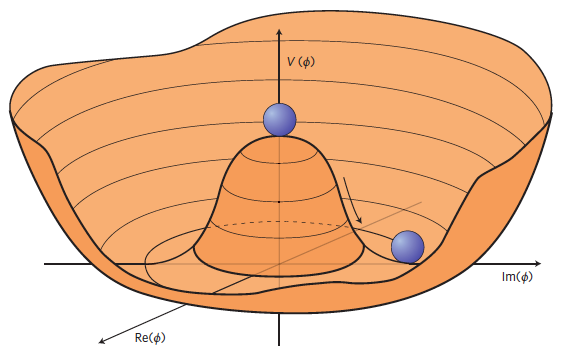
\includegraphics[scale=0.65]{figures/higgspotential}
\caption[The Higgs potential]{The Higgs potential.\cite{Ellis:1638469}}
\label{Fig:higgspot}
\end{center}
\end{figure}

\indent In QED, the four fundamental gauge bosons are ${W^{i}_{\mu}, i = 1,2,3}$ and ${B_{\mu}}$. These bosons couple to a complex scalar doublet, ${\Phi \equiv \binom{\phi^{+}}{\phi^{0}}}$. This doublet has a scalar potential.
\begin{equation}
\label{eq:higgsPot}
V(\Phi) = \mu^{2}|\Phi^{\dagger}\Phi| + \lambda(|\Phi^{\dagger}\Phi|)^{2}
\end{equation}
Where ${\mu^{2} < 0}$. This gives the Mexican hat shaped potential seen in figure ~\ref{Fig:higgspot}, with a minimum energy at 
\begin{equation}
\langle \phi \rangle = \sqrt{-\frac{\mu^{2}}{2\lambda}}\equiv \frac{\nu}{\sqrt{2}}
\end{equation}
called the vacuum expectation value (VEV) of ${\phi}$. The choice of the direction of fluctuation is arbitrary but can be chosen such that


 
\begin{equation}
\phi_{0} = \frac{1}{\sqrt{2}} \binom{0}{\nu}
\end{equation}
After the direction is chosen, the only remaining degree of freedom is the scalar field h(x), giving 
\begin{equation}
\phi(x) = \phi_{0} + h(x)
\end{equation}
The doublet can now be described by 
\begin{equation}
\Phi = \frac{1}{\sqrt{2}} \binom{0}{v+h(x)}
\end{equation}
This field couples to the gauge bosons as 
\begin{equation}
(\frac{g}{2}\overrightarrow{\tau}\cdot \overrightarrow{W} + \frac{g'}{2}B)\phi_{0}
\end{equation}
Where ${\overrightarrow{\tau}}$ are the Pauli matrices, ${\overrightarrow{W}}$ are ${W_{1,2,3}}$ and g, g' are the coupling constants. The result of the coupling is the acquisition of mass by three eigenstates of the bosons, 
\begin{equation}
\begin{split}
W^{\pm} = \frac{1}{\sqrt{2}}(W^{1}_{\mu} \mp iW^{2}_{\mu})\\
Z^{\mu} = \frac{-g'B_{\mu} + gW^{3}_{\mu}}{\sqrt{g^{2} + g'^{2}}}\\
A^{\mu} = \frac{gB_{\mu} + g'W^{3}_{\mu}}{\sqrt{g^{2} + g'^{2}}}
\end{split}
\end{equation}
These four eigenstates are the bosons we observe in the standard model. With Masses
\begin{equation}
\begin{split}
M^{2}_{W} = \frac{1}{4}g^{2}\nu^{2} \\
M^{2}_{Z} = \frac{1}{4}(g^{2} + g'^{2})\nu^{2} \\
M_{A} = 0
\end{split}
\end{equation}
Through the mixing that occurs in the spontaneous electroweak symmetry breaking gives mass to the standard model Gauge Bosons while leaving the photon, A, massless. However, for this to occur, an additional scalar field, the Higgs Field, is required.\newline
\indent The Higgs Boson is an excitation in the scalar Higgs field predicted in 1964~\cite{PhysRevLett.13.508}. The decay mechanism of this massive boson was predicted by Peter Higgs, allowing for the decay products to be measured. Giving a way to prove the existence of the scalar Higgs field. In 2012, a Higgs like scalar boson was discovered at the LHC by the ATLAS and CMS experiments with a mass of 125GeV/c\textsuperscript{2} ~\cite{Aad:2012tfa}.

\begin{figure}[h]
\begin{center}
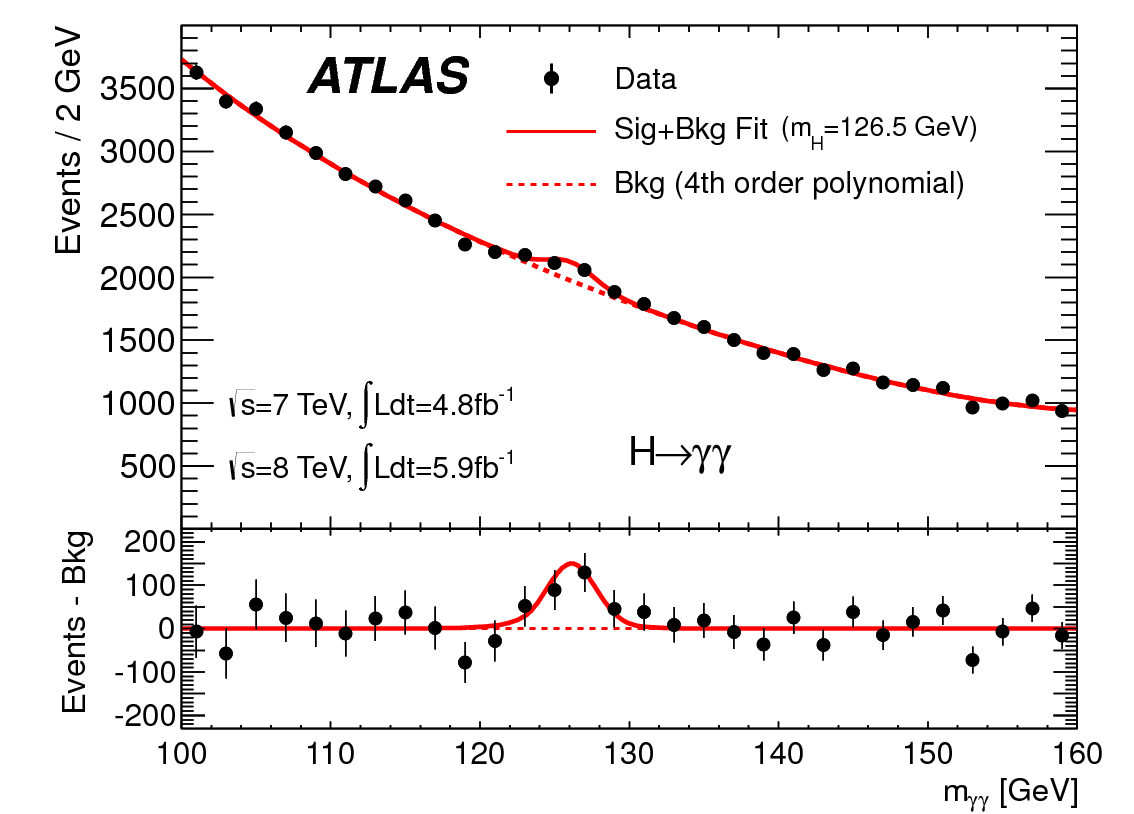
\includegraphics[scale=0.25]{figures/higgs_disc}
\caption[Higgs boson mass peak]{Invariant mass distribution of di-photon candidates for the combined root s = 7TeV and root s = 8TeV data samples. The result of a fit to the data of the sum of a signal component fixed to mH = 126.5GeV and a background component described by a fourth-order Bernstein polynomial is superimposed. The bottom inset displays the residuals of the data with respect to the fitted background component.}
\label{fig:Higgs}
\end{center}
\end{figure}

Since the discovery, many measurements have been made of this Higgs Boson to compare it to the standard model Higgs Boson. So far, the Higgs Boson has held up to these tests. The Higgs Boson has spin-parity J\textsuperscript{P} = 0\textsuperscript{+} ~\cite{Aad:2013xqa}, decays to bb ~\cite{Aaboud:2018zhk}, ${\gamma\gamma, \tau\tau}$ ~\cite{Aaboud:2018pen}, WW and ZZ have been measured with appropriate signal strengths, and no significant deviations have been observed in any Run 2 analyses. However, there are still many parameters of the Higgs Boson that still need measured. One of which is the triple Higgs coupling.
%Do I want to include more about the higgs discovery. 
